\documentclass[1p]{elsarticle_modified}
%\bibliographystyle{elsarticle-num}

%\usepackage[colorlinks]{hyperref}
%\usepackage{abbrmath_seonhwa} %\Abb, \Ascr, \Acal ,\Abf, \Afrak
\usepackage{amsfonts}
\usepackage{amssymb}
\usepackage{amsmath}
\usepackage{amsthm}
\usepackage{scalefnt}
\usepackage{amsbsy}
\usepackage{kotex}
\usepackage{caption}
\usepackage{subfig}
\usepackage{color}
\usepackage{graphicx}
\usepackage{xcolor} %% white, black, red, green, blue, cyan, magenta, yellow
\usepackage{float}
\usepackage{setspace}
\usepackage{hyperref}

\usepackage{tikz}
\usetikzlibrary{arrows}

\usepackage{multirow}
\usepackage{array} % fixed length table
\usepackage{hhline}

%%%%%%%%%%%%%%%%%%%%%
\makeatletter
\renewcommand*\env@matrix[1][\arraystretch]{%
	\edef\arraystretch{#1}%
	\hskip -\arraycolsep
	\let\@ifnextchar\new@ifnextchar
	\array{*\c@MaxMatrixCols c}}
\makeatother %https://tex.stackexchange.com/questions/14071/how-can-i-increase-the-line-spacing-in-a-matrix
%%%%%%%%%%%%%%%

\usepackage[normalem]{ulem}

\newcommand{\msout}[1]{\ifmmode\text{\sout{\ensuremath{#1}}}\else\sout{#1}\fi}
%SOURCE: \msout is \stkout macro in https://tex.stackexchange.com/questions/20609/strikeout-in-math-mode

\newcommand{\cancel}[1]{
	\ifmmode
	{\color{red}\msout{#1}}
	\else
	{\color{red}\sout{#1}}
	\fi
}

\newcommand{\add}[1]{
	{\color{blue}\uwave{#1}}
}

\newcommand{\replace}[2]{
	\ifmmode
	{\color{red}\msout{#1}}{\color{blue}\uwave{#2}}
	\else
	{\color{red}\sout{#1}}{\color{blue}\uwave{#2}}
	\fi
}

\newcommand{\Sol}{\mathcal{S}} %segment
\newcommand{\D}{D} %diagram
\newcommand{\A}{\mathcal{A}} %arc


%%%%%%%%%%%%%%%%%%%%%%%%%%%%%5 test

\def\sl{\operatorname{\textup{SL}}(2,\Cbb)}
\def\psl{\operatorname{\textup{PSL}}(2,\Cbb)}
\def\quan{\mkern 1mu \triangleright \mkern 1mu}

\theoremstyle{definition}
\newtheorem{thm}{Theorem}[section]
\newtheorem{prop}[thm]{Proposition}
\newtheorem{lem}[thm]{Lemma}
\newtheorem{ques}[thm]{Question}
\newtheorem{cor}[thm]{Corollary}
\newtheorem{defn}[thm]{Definition}
\newtheorem{exam}[thm]{Example}
\newtheorem{rmk}[thm]{Remark}
\newtheorem{alg}[thm]{Algorithm}

\newcommand{\I}{\sqrt{-1}}
\begin{document}

%\begin{frontmatter}
%
%\title{Boundary parabolic representations of knots up to 8 crossings}
%
%%% Group authors per affiliation:
%\author{Yunhi Cho} 
%\address{Department of Mathematics, University of Seoul, Seoul, Korea}
%\ead{yhcho@uos.ac.kr}
%
%
%\author{Seonhwa Kim} %\fnref{s_kim}}
%\address{Center for Geometry and Physics, Institute for Basic Science, Pohang, 37673, Korea}
%\ead{ryeona17@ibs.re.kr}
%
%\author{Hyuk Kim}
%\address{Department of Mathematical Sciences, Seoul National University, Seoul 08826, Korea}
%\ead{hyukkim@snu.ac.kr}
%
%\author{Seokbeom Yoon}
%\address{Department of Mathematical Sciences, Seoul National University, Seoul, 08826,  Korea}
%\ead{sbyoon15@snu.ac.kr}
%
%\begin{abstract}
%We find all boundary parabolic representation of knots up to 8 crossings.
%
%\end{abstract}
%\begin{keyword}
%    \MSC[2010] 57M25 
%\end{keyword}
%
%\end{frontmatter}

%\linenumbers
%\tableofcontents
%
\newcommand\colored[1]{\textcolor{white}{\rule[-0.35ex]{0.8em}{1.4ex}}\kern-0.8em\color{red} #1}%
%\newcommand\colored[1]{\textcolor{white}{ #1}\kern-2.17ex	\textcolor{white}{ #1}\kern-1.81ex	\textcolor{white}{ #1}\kern-2.15ex\color{red}#1	}

{\Large $\underline{11a_{312}~(K11a_{312})}$}

\setlength{\tabcolsep}{10pt}
\renewcommand{\arraystretch}{1.6}
\vspace{1cm}\begin{tabular}{m{100pt}>{\centering\arraybackslash}m{274pt}}
\multirow{5}{120pt}{
	\centering
	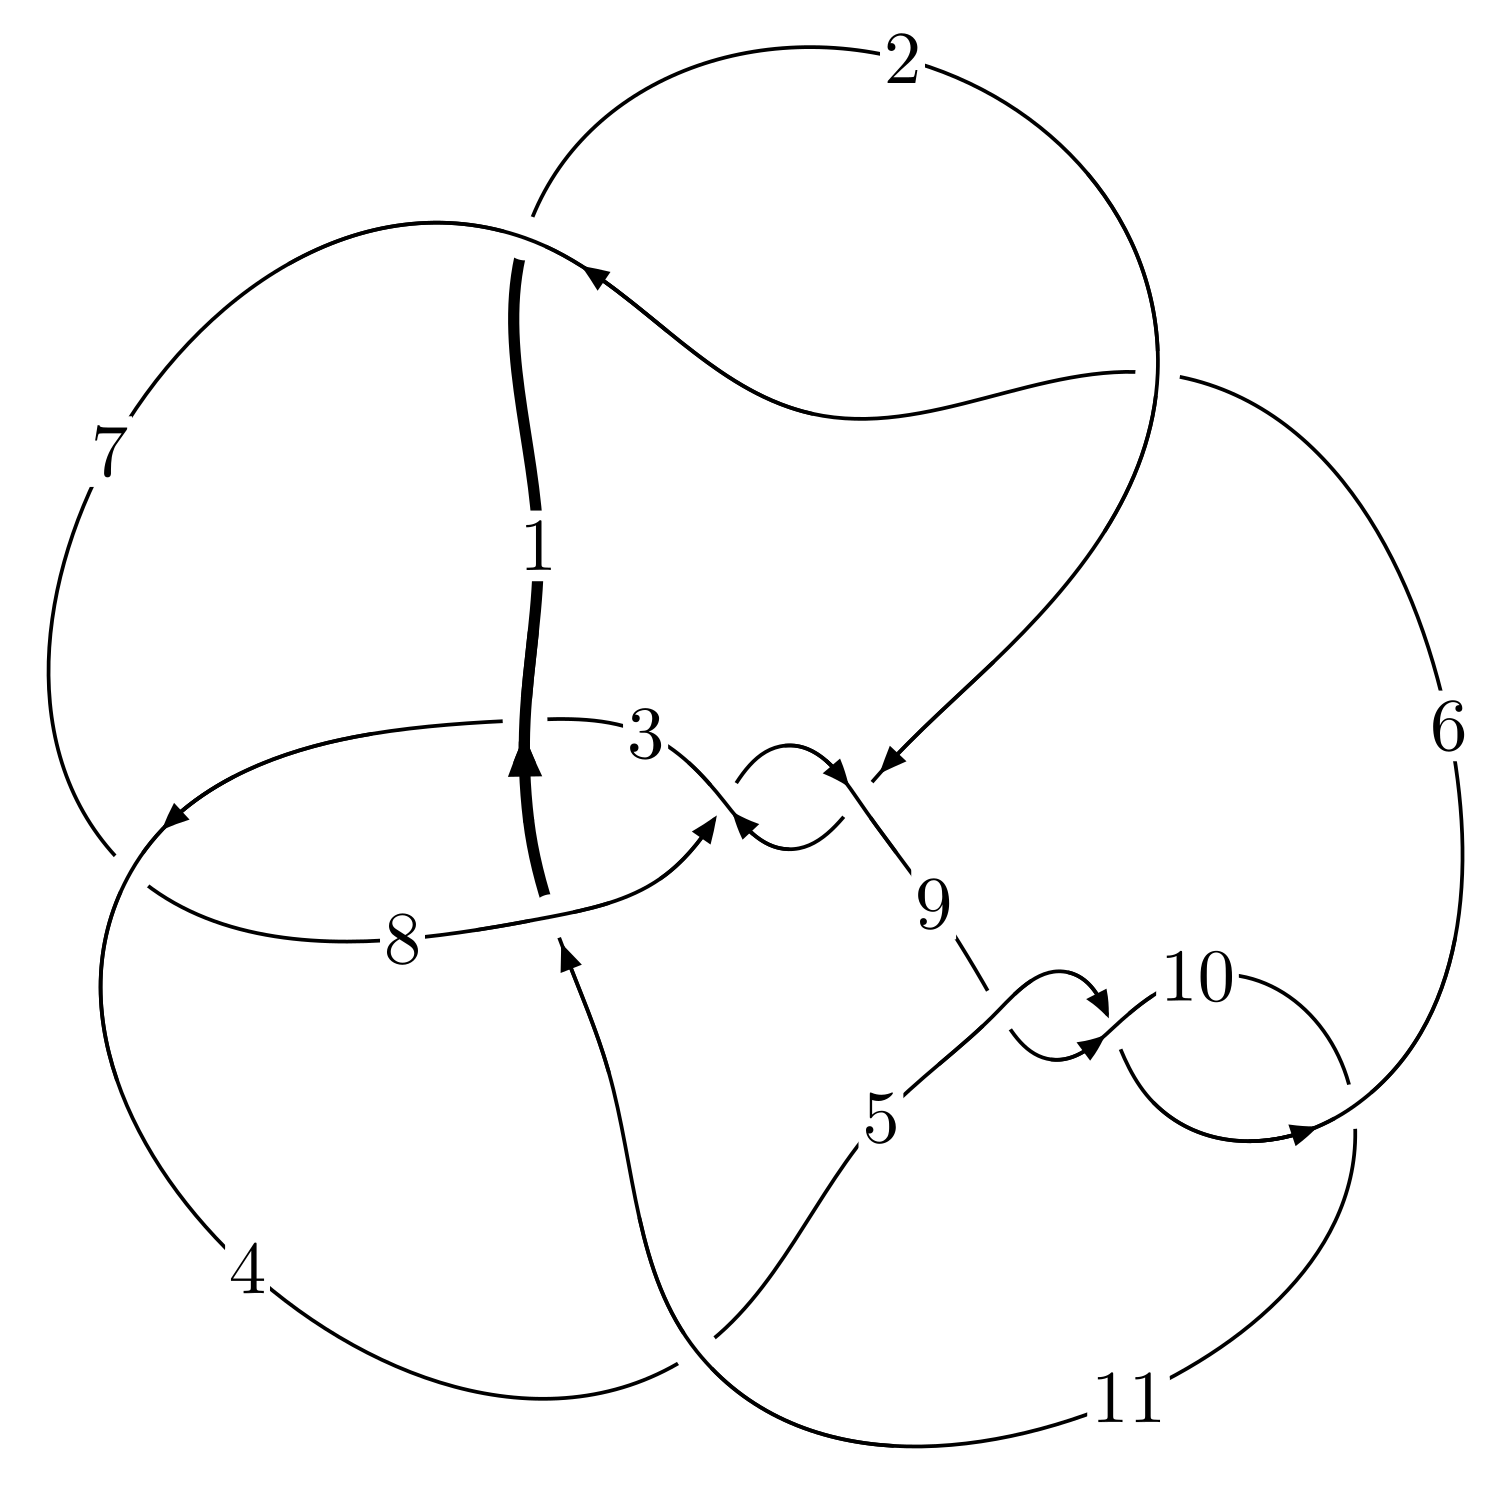
\includegraphics[width=112pt]{../../../GIT/diagram.site/Diagrams/png/561_11a_312.png}\\
\ \ \ A knot diagram\footnotemark}&
\allowdisplaybreaks
\textbf{Linearized knot diagam} \\
\cline{2-2}
 &
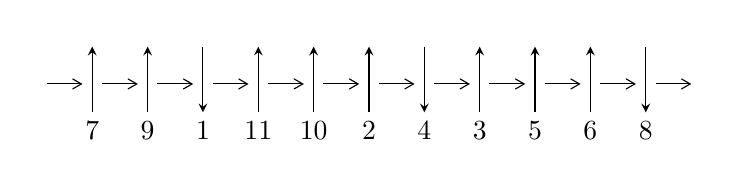
\begin{tikzpicture}[x=20pt, y=17pt]
	% nodes
	\node (C0) at (0, 0) {};
	\node (C1) at (1, 0) {};
	\node (C1U) at (1, +1) {};
	\node (C1D) at (1, -1) {7};

	\node (C2) at (2, 0) {};
	\node (C2U) at (2, +1) {};
	\node (C2D) at (2, -1) {9};

	\node (C3) at (3, 0) {};
	\node (C3U) at (3, +1) {};
	\node (C3D) at (3, -1) {1};

	\node (C4) at (4, 0) {};
	\node (C4U) at (4, +1) {};
	\node (C4D) at (4, -1) {11};

	\node (C5) at (5, 0) {};
	\node (C5U) at (5, +1) {};
	\node (C5D) at (5, -1) {10};

	\node (C6) at (6, 0) {};
	\node (C6U) at (6, +1) {};
	\node (C6D) at (6, -1) {2};

	\node (C7) at (7, 0) {};
	\node (C7U) at (7, +1) {};
	\node (C7D) at (7, -1) {4};

	\node (C8) at (8, 0) {};
	\node (C8U) at (8, +1) {};
	\node (C8D) at (8, -1) {3};

	\node (C9) at (9, 0) {};
	\node (C9U) at (9, +1) {};
	\node (C9D) at (9, -1) {5};

	\node (C10) at (10, 0) {};
	\node (C10U) at (10, +1) {};
	\node (C10D) at (10, -1) {6};

	\node (C11) at (11, 0) {};
	\node (C11U) at (11, +1) {};
	\node (C11D) at (11, -1) {8};
	\node (C12) at (12, 0) {};

	% arrows
	\draw[->,>={angle 60}]
	(C0) edge (C1) (C1) edge (C2) (C2) edge (C3) (C3) edge (C4) (C4) edge (C5) (C5) edge (C6) (C6) edge (C7) (C7) edge (C8) (C8) edge (C9) (C9) edge (C10) (C10) edge (C11) (C11) edge (C12) ;	\draw[->,>=stealth]
	(C1D) edge (C1U) (C2D) edge (C2U) (C3U) edge (C3D) (C4D) edge (C4U) (C5D) edge (C5U) (C6D) edge (C6U) (C7U) edge (C7D) (C8D) edge (C8U) (C9D) edge (C9U) (C10D) edge (C10U) (C11U) edge (C11D) ;
	\end{tikzpicture} \\
\hhline{~~} \\& 
\textbf{Solving Sequence} \\ \cline{2-2} 
 &
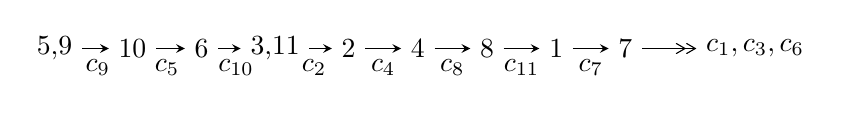
\begin{tikzpicture}[x=25pt, y=7pt]
	% node
	\node (A0) at (-1/8, 0) {5,9};
	\node (A1) at (1, 0) {10};
	\node (A2) at (2, 0) {6};
	\node (A3) at (49/16, 0) {3,11};
	\node (A4) at (33/8, 0) {2};
	\node (A5) at (41/8, 0) {4};
	\node (A6) at (49/8, 0) {8};
	\node (A7) at (57/8, 0) {1};
	\node (A8) at (65/8, 0) {7};
	\node (C1) at (1/2, -1) {$c_{9}$};
	\node (C2) at (3/2, -1) {$c_{5}$};
	\node (C3) at (5/2, -1) {$c_{10}$};
	\node (C4) at (29/8, -1) {$c_{2}$};
	\node (C5) at (37/8, -1) {$c_{4}$};
	\node (C6) at (45/8, -1) {$c_{8}$};
	\node (C7) at (53/8, -1) {$c_{11}$};
	\node (C8) at (61/8, -1) {$c_{7}$};
	\node (A9) at (10, 0) {$c_{1},c_{3},c_{6}$};

	% edge
	\draw[->,>=stealth]	
	(A0) edge (A1) (A1) edge (A2) (A2) edge (A3) (A3) edge (A4) (A4) edge (A5) (A5) edge (A6) (A6) edge (A7) (A7) edge (A8) ;
	\draw[->>,>={angle 60}]	
	(A8) edge (A9);
\end{tikzpicture} \\ 

\end{tabular} \\

\footnotetext{
The image of knot diagram is generated by the software ``\textbf{Draw programme}" developed by Andrew Bartholomew(\url{http://www.layer8.co.uk/maths/draw/index.htm\#Running-draw}), where we modified some parts for our purpose(\url{https://github.com/CATsTAILs/LinksPainter}).
}\phantom \\ \newline 
\centering \textbf{Ideals for irreducible components\footnotemark of $X_{\text{par}}$} 
 
\begin{align*}
I^u_{1}&=\langle 
73 u^{22}+403 u^{21}+\cdots+4 b-388,\;13 u^{22}+105 u^{21}+\cdots+8 a-196,\;u^{23}+7 u^{22}+\cdots+20 u-8\rangle \\
I^u_{2}&=\langle 
-23118805228540 u^7 a^5+8120163058708 u^7 a^4+\cdots+167668012322500 a+126864012582143,\\
\phantom{I^u_{2}}&\phantom{= \langle  }-2 u^7 a^5-3 u^7 a^4+\cdots+54 a+10,\;u^8- u^7-3 u^6+2 u^5+3 u^4-2 u-1\rangle \\
I^u_{3}&=\langle 
u^{11}-5 u^9+8 u^7+u^6-2 u^5-3 u^4-4 u^3+2 u^2+b+u,\\
\phantom{I^u_{3}}&\phantom{= \langle  }- u^{10}- u^9+4 u^8+4 u^7-4 u^6-5 u^5-3 u^4+4 u^2+a+3 u+2,\\
\phantom{I^u_{3}}&\phantom{= \langle  }u^{12}-6 u^{10}+13 u^8+u^7-10 u^6-4 u^5-2 u^4+5 u^3+4 u^2-2 u+1\rangle \\
\\
\end{align*}
\raggedright * 3 irreducible components of $\dim_{\mathbb{C}}=0$, with total 83 representations.\\
\footnotetext{All coefficients of polynomials are rational numbers. But the coefficients are sometimes approximated in decimal forms when there is not enough margin.}
\newpage
\renewcommand{\arraystretch}{1}
\centering \section*{I. $I^u_{1}= \langle 73 u^{22}+403 u^{21}+\cdots+4 b-388,\;13 u^{22}+105 u^{21}+\cdots+8 a-196,\;u^{23}+7 u^{22}+\cdots+20 u-8 \rangle$}
\flushleft \textbf{(i) Arc colorings}\\
\begin{tabular}{m{7pt} m{180pt} m{7pt} m{180pt} }
\flushright $a_{5}=$&$\begin{pmatrix}0\\u\end{pmatrix}$ \\
\flushright $a_{9}=$&$\begin{pmatrix}1\\0\end{pmatrix}$ \\
\flushright $a_{10}=$&$\begin{pmatrix}1\\- u^2\end{pmatrix}$ \\
\flushright $a_{6}=$&$\begin{pmatrix}u\\- u^3+u\end{pmatrix}$ \\
\flushright $a_{3}=$&$\begin{pmatrix}-1.62500 u^{22}-13.1250 u^{21}+\cdots-88.7500 u+24.5000\\-\frac{73}{4} u^{22}-\frac{403}{4} u^{21}+\cdots-303 u+97\end{pmatrix}$ \\
\flushright $a_{11}=$&$\begin{pmatrix}- u^2+1\\u^4-2 u^2\end{pmatrix}$ \\
\flushright $a_{2}=$&$\begin{pmatrix}16.6250 u^{22}+87.6250 u^{21}+\cdots+214.250 u-72.5000\\-\frac{73}{4} u^{22}-\frac{403}{4} u^{21}+\cdots-303 u+97\end{pmatrix}$ \\
\flushright $a_{4}=$&$\begin{pmatrix}- u^5+2 u^3- u\\u^7-3 u^5+2 u^3+u\end{pmatrix}$ \\
\flushright $a_{8}=$&$\begin{pmatrix}-\frac{93}{8} u^{22}-\frac{517}{8} u^{21}+\cdots-\frac{769}{4} u+62\\\frac{37}{4} u^{22}+\frac{213}{4} u^{21}+\cdots+\frac{389}{2} u-59\end{pmatrix}$ \\
\flushright $a_{1}=$&$\begin{pmatrix}-\frac{13}{8} u^{22}-\frac{67}{8} u^{21}+\cdots-21 u+8\\-\frac{19}{2} u^{22}-55 u^{21}+\cdots-\frac{383}{2} u+59\end{pmatrix}$ \\
\flushright $a_{7}=$&$\begin{pmatrix}\frac{167}{8} u^{22}+\frac{943}{8} u^{21}+\cdots+\frac{1551}{4} u-120\\-\frac{37}{4} u^{22}-\frac{213}{4} u^{21}+\cdots-\frac{387}{2} u+59\end{pmatrix}$\\ \flushright $a_{7}=$&$\begin{pmatrix}\frac{167}{8} u^{22}+\frac{943}{8} u^{21}+\cdots+\frac{1551}{4} u-120\\-\frac{37}{4} u^{22}-\frac{213}{4} u^{21}+\cdots-\frac{387}{2} u+59\end{pmatrix}$\\&\end{tabular}
\flushleft \textbf{(ii) Obstruction class $= -1$}\\~\\
\flushleft \textbf{(iii) Cusp Shapes $= 3 u^{22}+17 u^{21}+24 u^{20}-24 u^{19}-51 u^{18}+70 u^{17}+81 u^{16}-139 u^{15}+10 u^{14}+241 u^{13}-226 u^{12}-212 u^{11}+397 u^{10}-84 u^9-335 u^8+295 u^7-62 u^6-302 u^5+136 u^4-15 u^3-78 u^2+40 u-2$}\\~\\
\newpage\renewcommand{\arraystretch}{1}
\flushleft \textbf{(iv) u-Polynomials at the component}\newline \\
\begin{tabular}{m{50pt}|m{274pt}}
Crossings & \hspace{64pt}u-Polynomials at each crossing \\
\hline $$\begin{aligned}c_{1},c_{2},c_{6}\\c_{8}\end{aligned}$$&$\begin{aligned}
&u^{23}+10 u^{21}+\cdots+3 u-1
\end{aligned}$\\
\hline $$\begin{aligned}c_{3}\end{aligned}$$&$\begin{aligned}
&u^{23}-24 u^{22}+\cdots+3840 u-256
\end{aligned}$\\
\hline $$\begin{aligned}c_{4}\end{aligned}$$&$\begin{aligned}
&u^{23}-21 u^{22}+\cdots-11268 u+1192
\end{aligned}$\\
\hline $$\begin{aligned}c_{5},c_{9},c_{10}\end{aligned}$$&$\begin{aligned}
&u^{23}+7 u^{22}+\cdots+20 u-8
\end{aligned}$\\
\hline $$\begin{aligned}c_{7},c_{11}\end{aligned}$$&$\begin{aligned}
&u^{23}+u^{22}+\cdots+3 u^2-1
\end{aligned}$\\
\hline
\end{tabular}\\~\\
\newpage\renewcommand{\arraystretch}{1}
\flushleft \textbf{(v) Riley Polynomials at the component}\newline \\
\begin{tabular}{m{50pt}|m{274pt}}
Crossings & \hspace{64pt}Riley Polynomials at each crossing \\
\hline $$\begin{aligned}c_{1},c_{2},c_{6}\\c_{8}\end{aligned}$$&$\begin{aligned}
&y^{23}+20 y^{22}+\cdots+13 y-1
\end{aligned}$\\
\hline $$\begin{aligned}c_{3}\end{aligned}$$&$\begin{aligned}
&y^{23}-4 y^{22}+\cdots+131072 y-65536
\end{aligned}$\\
\hline $$\begin{aligned}c_{4}\end{aligned}$$&$\begin{aligned}
&y^{23}+9 y^{22}+\cdots+19115664 y-1420864
\end{aligned}$\\
\hline $$\begin{aligned}c_{5},c_{9},c_{10}\end{aligned}$$&$\begin{aligned}
&y^{23}-19 y^{22}+\cdots+144 y-64
\end{aligned}$\\
\hline $$\begin{aligned}c_{7},c_{11}\end{aligned}$$&$\begin{aligned}
&y^{23}-3 y^{22}+\cdots+6 y-1
\end{aligned}$\\
\hline
\end{tabular}\\~\\
\newpage\flushleft \textbf{(vi) Complex Volumes and Cusp Shapes}
$$\begin{array}{c|c|c}  
\text{Solutions to }I^u_{1}& \I (\text{vol} + \sqrt{-1}CS) & \text{Cusp shape}\\
 \hline 
\begin{aligned}
u &= \phantom{-}0.293135 + 1.025030 I \\
a &= \phantom{-}0.46656 - 1.57304 I \\
b &= -0.147192 - 1.229000 I\end{aligned}
 & -7.64064 + 1.90172 I & -11.16155 - 1.95097 I \\ \hline\begin{aligned}
u &= \phantom{-}0.293135 - 1.025030 I \\
a &= \phantom{-}0.46656 + 1.57304 I \\
b &= -0.147192 + 1.229000 I\end{aligned}
 & -7.64064 - 1.90172 I & -11.16155 + 1.95097 I \\ \hline\begin{aligned}
u &= \phantom{-}0.202954 + 0.883680 I \\
a &= -0.38232 + 2.26017 I \\
b &= \phantom{-}0.48719 + 1.49237 I\end{aligned}
 & -9.7130 + 11.5082 I & -0.75618 - 6.89858 I \\ \hline\begin{aligned}
u &= \phantom{-}0.202954 - 0.883680 I \\
a &= -0.38232 - 2.26017 I \\
b &= \phantom{-}0.48719 - 1.49237 I\end{aligned}
 & -9.7130 - 11.5082 I & -0.75618 + 6.89858 I \\ \hline\begin{aligned}
u &= \phantom{-}0.881214 + 0.717683 I \\
a &= \phantom{-}0.446178 - 1.010460 I \\
b &= -0.044762 - 1.270850 I\end{aligned}
 & -5.82775 + 3.98753 I & -2.21274 - 8.17133 I \\ \hline\begin{aligned}
u &= \phantom{-}0.881214 - 0.717683 I \\
a &= \phantom{-}0.446178 + 1.010460 I \\
b &= -0.044762 + 1.270850 I\end{aligned}
 & -5.82775 - 3.98753 I & -2.21274 + 8.17133 I \\ \hline\begin{aligned}
u &= \phantom{-}1.14836\phantom{ +0.000000I} \\
a &= \phantom{-}0.267977\phantom{ +0.000000I} \\
b &= \phantom{-}0.450637\phantom{ +0.000000I}\end{aligned}
 & \phantom{-}1.73407\phantom{ +0.000000I} & \phantom{-}6.87040\phantom{ +0.000000I} \\ \hline\begin{aligned}
u &= \phantom{-}1.034490 + 0.522098 I \\
a &= -0.652102 + 0.902922 I \\
b &= -0.37473 + 1.45394 I\end{aligned}
 & -7.16797 - 6.55570 I & \phantom{-}1.22391 + 3.26324 I \\ \hline\begin{aligned}
u &= \phantom{-}1.034490 - 0.522098 I \\
a &= -0.652102 - 0.902922 I \\
b &= -0.37473 - 1.45394 I\end{aligned}
 & -7.16797 + 6.55570 I & \phantom{-}1.22391 - 3.26324 I \\ \hline\begin{aligned}
u &= \phantom{-}0.232269 + 0.616489 I \\
a &= -0.683421 - 0.586793 I \\
b &= -0.575175 + 0.039007 I\end{aligned}
 & -0.29865 + 2.39912 I & \phantom{-}6.29196 - 4.13143 I\\
 \hline 
 \end{array}$$\newpage$$\begin{array}{c|c|c}  
\text{Solutions to }I^u_{1}& \I (\text{vol} + \sqrt{-1}CS) & \text{Cusp shape}\\
 \hline 
\begin{aligned}
u &= \phantom{-}0.232269 - 0.616489 I \\
a &= -0.683421 + 0.586793 I \\
b &= -0.575175 - 0.039007 I\end{aligned}
 & -0.29865 - 2.39912 I & \phantom{-}6.29196 + 4.13143 I \\ \hline\begin{aligned}
u &= -1.372390 + 0.114615 I \\
a &= \phantom{-}0.820986 + 0.214490 I \\
b &= -0.737153 + 0.407888 I\end{aligned}
 & \phantom{-}6.36396 - 1.94185 I & \phantom{-}12.44424 + 2.77963 I \\ \hline\begin{aligned}
u &= -1.372390 - 0.114615 I \\
a &= \phantom{-}0.820986 - 0.214490 I \\
b &= -0.737153 - 0.407888 I\end{aligned}
 & \phantom{-}6.36396 + 1.94185 I & \phantom{-}12.44424 - 2.77963 I \\ \hline\begin{aligned}
u &= -1.381230 + 0.237993 I \\
a &= -0.152679 - 0.704144 I \\
b &= \phantom{-}0.670861 - 0.027425 I\end{aligned}
 & \phantom{-}4.83020 - 5.52175 I & \phantom{-}12.07498 + 4.89921 I \\ \hline\begin{aligned}
u &= -1.381230 - 0.237993 I \\
a &= -0.152679 + 0.704144 I \\
b &= \phantom{-}0.670861 + 0.027425 I\end{aligned}
 & \phantom{-}4.83020 + 5.52175 I & \phantom{-}12.07498 - 4.89921 I \\ \hline\begin{aligned}
u &= -1.39795 + 0.37738 I \\
a &= \phantom{-}1.40129 + 1.12721 I \\
b &= -0.57325 + 1.48723 I\end{aligned}
 & -4.6506 - 16.0409 I & \phantom{-}3.32343 + 8.47375 I \\ \hline\begin{aligned}
u &= -1.39795 - 0.37738 I \\
a &= \phantom{-}1.40129 - 1.12721 I \\
b &= -0.57325 - 1.48723 I\end{aligned}
 & -4.6506 + 16.0409 I & \phantom{-}3.32343 - 8.47375 I \\ \hline\begin{aligned}
u &= -1.42052 + 0.45491 I \\
a &= -0.968130 - 0.943346 I \\
b &= \phantom{-}0.318171 - 1.163070 I\end{aligned}
 & -2.31364 - 7.21005 I & -0.81443 + 11.11700 I \\ \hline\begin{aligned}
u &= -1.42052 - 0.45491 I \\
a &= -0.968130 + 0.943346 I \\
b &= \phantom{-}0.318171 + 1.163070 I\end{aligned}
 & -2.31364 + 7.21005 I & -0.81443 - 11.11700 I \\ \hline\begin{aligned}
u &= \phantom{-}0.401495 + 0.274693 I \\
a &= -0.290970 + 0.483465 I \\
b &= \phantom{-}0.473749 + 0.279232 I\end{aligned}
 & \phantom{-}0.892504 + 0.454173 I & \phantom{-}10.11280 - 4.18130 I\\
 \hline 
 \end{array}$$\newpage$$\begin{array}{c|c|c}  
\text{Solutions to }I^u_{1}& \I (\text{vol} + \sqrt{-1}CS) & \text{Cusp shape}\\
 \hline 
\begin{aligned}
u &= \phantom{-}0.401495 - 0.274693 I \\
a &= -0.290970 - 0.483465 I \\
b &= \phantom{-}0.473749 - 0.279232 I\end{aligned}
 & \phantom{-}0.892504 - 0.454173 I & \phantom{-}10.11280 + 4.18130 I \\ \hline\begin{aligned}
u &= -1.54765 + 0.11437 I \\
a &= -0.389379 + 0.033075 I \\
b &= \phantom{-}0.276976 - 1.131580 I\end{aligned}
 & \phantom{-}2.45199 - 6.58203 I & \phantom{-}4.53835 + 6.99896 I \\ \hline\begin{aligned}
u &= -1.54765 - 0.11437 I \\
a &= -0.389379 - 0.033075 I \\
b &= \phantom{-}0.276976 + 1.131580 I\end{aligned}
 & \phantom{-}2.45199 + 6.58203 I & \phantom{-}4.53835 - 6.99896 I\\
 \hline 
 \end{array}$$\newpage\newpage\renewcommand{\arraystretch}{1}
\centering \section*{II. $I^u_{2}= \langle -2.31\times10^{13} a^{5} u^{7}+8.12\times10^{12} a^{4} u^{7}+\cdots+1.68\times10^{14} a+1.27\times10^{14},\;-2 u^7 a^5-3 u^7 a^4+\cdots+54 a+10,\;u^8- u^7-3 u^6+2 u^5+3 u^4-2 u-1 \rangle$}
\flushleft \textbf{(i) Arc colorings}\\
\begin{tabular}{m{7pt} m{180pt} m{7pt} m{180pt} }
\flushright $a_{5}=$&$\begin{pmatrix}0\\u\end{pmatrix}$ \\
\flushright $a_{9}=$&$\begin{pmatrix}1\\0\end{pmatrix}$ \\
\flushright $a_{10}=$&$\begin{pmatrix}1\\- u^2\end{pmatrix}$ \\
\flushright $a_{6}=$&$\begin{pmatrix}u\\- u^3+u\end{pmatrix}$ \\
\flushright $a_{3}=$&$\begin{pmatrix}a\\0.392427 a^{5} u^{7}-0.137835 a^{4} u^{7}+\cdots-2.84606 a-2.15344\end{pmatrix}$ \\
\flushright $a_{11}=$&$\begin{pmatrix}- u^2+1\\u^4-2 u^2\end{pmatrix}$ \\
\flushright $a_{2}=$&$\begin{pmatrix}-0.392427 a^{5} u^{7}+0.137835 a^{4} u^{7}+\cdots+3.84606 a+2.15344\\0.392427 a^{5} u^{7}-0.137835 a^{4} u^{7}+\cdots-2.84606 a-2.15344\end{pmatrix}$ \\
\flushright $a_{4}=$&$\begin{pmatrix}- u^5+2 u^3- u\\u^7-3 u^5+2 u^3+u\end{pmatrix}$ \\
\flushright $a_{8}=$&$\begin{pmatrix}0.619590 a^{5} u^{7}+0.411741 a^{4} u^{7}+\cdots+5.96004 a+6.04257\\-0.461898 a^{5} u^{7}+0.617791 a^{4} u^{7}+\cdots-2.20681 a-0.962589\end{pmatrix}$ \\
\flushright $a_{1}=$&$\begin{pmatrix}0.863277 a^{5} u^{7}+0.0511046 a^{4} u^{7}+\cdots-1.95851 a-2.40659\\-1.09603 a^{5} u^{7}-0.183794 a^{4} u^{7}+\cdots-3.37057 a-1.13036\end{pmatrix}$ \\
\flushright $a_{7}=$&$\begin{pmatrix}0.257408 a^{5} u^{7}-0.257217 a^{4} u^{7}+\cdots+8.19095 a+7.33644\\-0.388740 a^{5} u^{7}+0.461509 a^{4} u^{7}+\cdots-4.45800 a-2.53941\end{pmatrix}$\\ \flushright $a_{7}=$&$\begin{pmatrix}0.257408 a^{5} u^{7}-0.257217 a^{4} u^{7}+\cdots+8.19095 a+7.33644\\-0.388740 a^{5} u^{7}+0.461509 a^{4} u^{7}+\cdots-4.45800 a-2.53941\end{pmatrix}$\\&\end{tabular}
\flushleft \textbf{(ii) Obstruction class $= -1$}\\~\\
\flushleft \textbf{(iii) Cusp Shapes $= -\frac{17781823578608}{58912383397937} u^7 a^5+\frac{890888304264}{58912383397937} u^7 a^4+\cdots-\frac{483633451308792}{58912383397937} a-\frac{241926483811578}{58912383397937}$}\\~\\
\newpage\renewcommand{\arraystretch}{1}
\flushleft \textbf{(iv) u-Polynomials at the component}\newline \\
\begin{tabular}{m{50pt}|m{274pt}}
Crossings & \hspace{64pt}u-Polynomials at each crossing \\
\hline $$\begin{aligned}c_{1},c_{2},c_{6}\\c_{8}\end{aligned}$$&$\begin{aligned}
&u^{48}+u^{47}+\cdots+160 u+293
\end{aligned}$\\
\hline $$\begin{aligned}c_{3}\end{aligned}$$&$\begin{aligned}
&(u^3+u^2-1)^{16}
\end{aligned}$\\
\hline $$\begin{aligned}c_{4}\end{aligned}$$&$\begin{aligned}
&(u^8+3 u^7+7 u^6+10 u^5+11 u^4+10 u^3+6 u^2+4 u+1)^6
\end{aligned}$\\
\hline $$\begin{aligned}c_{5},c_{9},c_{10}\end{aligned}$$&$\begin{aligned}
&(u^8- u^7-3 u^6+2 u^5+3 u^4-2 u-1)^6
\end{aligned}$\\
\hline $$\begin{aligned}c_{7},c_{11}\end{aligned}$$&$\begin{aligned}
&u^{48}+3 u^{47}+\cdots+890 u+173
\end{aligned}$\\
\hline
\end{tabular}\\~\\
\newpage\renewcommand{\arraystretch}{1}
\flushleft \textbf{(v) Riley Polynomials at the component}\newline \\
\begin{tabular}{m{50pt}|m{274pt}}
Crossings & \hspace{64pt}Riley Polynomials at each crossing \\
\hline $$\begin{aligned}c_{1},c_{2},c_{6}\\c_{8}\end{aligned}$$&$\begin{aligned}
&y^{48}+39 y^{47}+\cdots-564720 y+85849
\end{aligned}$\\
\hline $$\begin{aligned}c_{3}\end{aligned}$$&$\begin{aligned}
&(y^3- y^2+2 y-1)^{16}
\end{aligned}$\\
\hline $$\begin{aligned}c_{4}\end{aligned}$$&$\begin{aligned}
&(y^8+5 y^7+11 y^6+6 y^5-17 y^4-34 y^3-22 y^2-4 y+1)^6
\end{aligned}$\\
\hline $$\begin{aligned}c_{5},c_{9},c_{10}\end{aligned}$$&$\begin{aligned}
&(y^8-7 y^7+19 y^6-22 y^5+3 y^4+14 y^3-6 y^2-4 y+1)^6
\end{aligned}$\\
\hline $$\begin{aligned}c_{7},c_{11}\end{aligned}$$&$\begin{aligned}
&y^{48}-13 y^{47}+\cdots-826008 y+29929
\end{aligned}$\\
\hline
\end{tabular}\\~\\
\newpage\flushleft \textbf{(vi) Complex Volumes and Cusp Shapes}
$$\begin{array}{c|c|c}  
\text{Solutions to }I^u_{2}& \I (\text{vol} + \sqrt{-1}CS) & \text{Cusp shape}\\
 \hline 
\begin{aligned}
u &= -1.180120 + 0.268597 I \\
a &= -0.896822 - 0.641304 I \\
b &= -0.44089 - 1.82899 I\end{aligned}
 & -5.00760 - 1.13123 I & -3.60429 + 0.51079 I \\ \hline\begin{aligned}
u &= -1.180120 + 0.268597 I \\
a &= -0.989164 - 0.528833 I \\
b &= \phantom{-}0.347952 + 0.310629 I\end{aligned}
 & -0.87002 - 3.95936 I & \phantom{-}2.92498 + 3.49024 I \\ \hline\begin{aligned}
u &= -1.180120 + 0.268597 I \\
a &= \phantom{-}0.141663 + 0.835373 I \\
b &= -1.167430 - 0.563919 I\end{aligned}
 & -0.87002 + 1.69689 I & \phantom{-}2.92498 - 2.46866 I \\ \hline\begin{aligned}
u &= -1.180120 + 0.268597 I \\
a &= -0.123278 + 1.382340 I \\
b &= \phantom{-}0.11559 + 1.41262 I\end{aligned}
 & -5.00760 - 1.13123 I & -3.60429 + 0.51079 I \\ \hline\begin{aligned}
u &= -1.180120 + 0.268597 I \\
a &= -1.09571 - 1.53145 I \\
b &= \phantom{-}0.484357 - 1.213990 I\end{aligned}
 & -0.87002 - 3.95936 I & \phantom{-}2.92498 + 3.49024 I \\ \hline\begin{aligned}
u &= -1.180120 + 0.268597 I \\
a &= \phantom{-}1.17316 + 1.78430 I \\
b &= \phantom{-}0.089556 + 1.152970 I\end{aligned}
 & -0.87002 + 1.69689 I & \phantom{-}2.92498 - 2.46866 I \\ \hline\begin{aligned}
u &= -1.180120 - 0.268597 I \\
a &= -0.896822 + 0.641304 I \\
b &= -0.44089 + 1.82899 I\end{aligned}
 & -5.00760 + 1.13123 I & -3.60429 - 0.51079 I \\ \hline\begin{aligned}
u &= -1.180120 - 0.268597 I \\
a &= -0.989164 + 0.528833 I \\
b &= \phantom{-}0.347952 - 0.310629 I\end{aligned}
 & -0.87002 + 3.95936 I & \phantom{-}2.92498 - 3.49024 I \\ \hline\begin{aligned}
u &= -1.180120 - 0.268597 I \\
a &= \phantom{-}0.141663 - 0.835373 I \\
b &= -1.167430 + 0.563919 I\end{aligned}
 & -0.87002 - 1.69689 I & \phantom{-}2.92498 + 2.46866 I \\ \hline\begin{aligned}
u &= -1.180120 - 0.268597 I \\
a &= -0.123278 - 1.382340 I \\
b &= \phantom{-}0.11559 - 1.41262 I\end{aligned}
 & -5.00760 + 1.13123 I & -3.60429 - 0.51079 I\\
 \hline 
 \end{array}$$\newpage$$\begin{array}{c|c|c}  
\text{Solutions to }I^u_{2}& \I (\text{vol} + \sqrt{-1}CS) & \text{Cusp shape}\\
 \hline 
\begin{aligned}
u &= -1.180120 - 0.268597 I \\
a &= -1.09571 + 1.53145 I \\
b &= \phantom{-}0.484357 + 1.213990 I\end{aligned}
 & -0.87002 + 3.95936 I & \phantom{-}2.92498 - 3.49024 I \\ \hline\begin{aligned}
u &= -1.180120 - 0.268597 I \\
a &= \phantom{-}1.17316 - 1.78430 I \\
b &= \phantom{-}0.089556 - 1.152970 I\end{aligned}
 & -0.87002 - 1.69689 I & \phantom{-}2.92498 + 2.46866 I \\ \hline\begin{aligned}
u &= -0.108090 + 0.747508 I \\
a &= \phantom{-}1.012830 - 0.490873 I \\
b &= \phantom{-}1.294730 - 0.286176 I\end{aligned}
 & -4.07009 - 5.40662 I & -0.21317 + 6.54740 I \\ \hline\begin{aligned}
u &= -0.108090 + 0.747508 I \\
a &= \phantom{-}0.192080 - 0.476649 I \\
b &= -0.465784 - 0.043673 I\end{aligned}
 & -4.07009 + 0.24963 I & -0.213168 + 0.588510 I \\ \hline\begin{aligned}
u &= -0.108090 + 0.747508 I \\
a &= -0.50426 - 2.37465 I \\
b &= -0.220687 - 1.217460 I\end{aligned}
 & -4.07009 + 0.24963 I & -0.213168 + 0.588510 I \\ \hline\begin{aligned}
u &= -0.108090 + 0.747508 I \\
a &= -0.12907 - 2.65292 I \\
b &= \phantom{-}0.66006 - 1.66847 I\end{aligned}
 & -8.20767 - 2.57849 I & -6.74243 + 3.56796 I \\ \hline\begin{aligned}
u &= -0.108090 + 0.747508 I \\
a &= \phantom{-}1.31751 + 2.32128 I \\
b &= -0.172710 + 1.289020 I\end{aligned}
 & -8.20767 - 2.57849 I & -6.74243 + 3.56796 I \\ \hline\begin{aligned}
u &= -0.108090 + 0.747508 I \\
a &= \phantom{-}0.19648 + 3.09182 I \\
b &= -0.240367 + 1.260870 I\end{aligned}
 & -4.07009 - 5.40662 I & -0.21317 + 6.54740 I \\ \hline\begin{aligned}
u &= -0.108090 - 0.747508 I \\
a &= \phantom{-}1.012830 + 0.490873 I \\
b &= \phantom{-}1.294730 + 0.286176 I\end{aligned}
 & -4.07009 + 5.40662 I & -0.21317 - 6.54740 I \\ \hline\begin{aligned}
u &= -0.108090 - 0.747508 I \\
a &= \phantom{-}0.192080 + 0.476649 I \\
b &= -0.465784 + 0.043673 I\end{aligned}
 & -4.07009 - 0.24963 I & -0.213168 - 0.588510 I\\
 \hline 
 \end{array}$$\newpage$$\begin{array}{c|c|c}  
\text{Solutions to }I^u_{2}& \I (\text{vol} + \sqrt{-1}CS) & \text{Cusp shape}\\
 \hline 
\begin{aligned}
u &= -0.108090 - 0.747508 I \\
a &= -0.50426 + 2.37465 I \\
b &= -0.220687 + 1.217460 I\end{aligned}
 & -4.07009 - 0.24963 I & -0.213168 - 0.588510 I \\ \hline\begin{aligned}
u &= -0.108090 - 0.747508 I \\
a &= -0.12907 + 2.65292 I \\
b &= \phantom{-}0.66006 + 1.66847 I\end{aligned}
 & -8.20767 + 2.57849 I & -6.74243 - 3.56796 I \\ \hline\begin{aligned}
u &= -0.108090 - 0.747508 I \\
a &= \phantom{-}1.31751 - 2.32128 I \\
b &= -0.172710 - 1.289020 I\end{aligned}
 & -8.20767 + 2.57849 I & -6.74243 - 3.56796 I \\ \hline\begin{aligned}
u &= -0.108090 - 0.747508 I \\
a &= \phantom{-}0.19648 - 3.09182 I \\
b &= -0.240367 - 1.260870 I\end{aligned}
 & -4.07009 + 5.40662 I & -0.21317 - 6.54740 I \\ \hline\begin{aligned}
u &= \phantom{-}1.37100\phantom{ +0.000000I} \\
a &= \phantom{-}0.216638 + 0.976013 I \\
b &= \phantom{-}0.312893 - 1.010360 I\end{aligned}
 & \phantom{-}0.454474\phantom{ +0.000000I} & \phantom{-}2.84453 + 0. I\phantom{ +0.000000I} \\ \hline\begin{aligned}
u &= \phantom{-}1.37100\phantom{ +0.000000I} \\
a &= \phantom{-}0.216638 - 0.976013 I \\
b &= \phantom{-}0.312893 + 1.010360 I\end{aligned}
 & \phantom{-}0.454474\phantom{ +0.000000I} & \phantom{-}2.84453 + 0. I\phantom{ +0.000000I} \\ \hline\begin{aligned}
u &= \phantom{-}1.37100\phantom{ +0.000000I} \\
a &= -0.567976 + 0.778979 I \\
b &= \phantom{-}0.790704 + 0.425774 I\end{aligned}
 & \phantom{-}4.59206 - 2.82812 I & \phantom{-}9.37379 + 2.97945 I \\ \hline\begin{aligned}
u &= \phantom{-}1.37100\phantom{ +0.000000I} \\
a &= -0.567976 - 0.778979 I \\
b &= \phantom{-}0.790704 - 0.425774 I\end{aligned}
 & \phantom{-}4.59206 + 2.82812 I & \phantom{-}9.37379 - 2.97945 I \\ \hline\begin{aligned}
u &= \phantom{-}1.37100\phantom{ +0.000000I} \\
a &= \phantom{-}0.731511 + 0.214900 I \\
b &= -0.554508 + 1.009700 I\end{aligned}
 & \phantom{-}4.59206 - 2.82812 I & \phantom{-}9.37379 + 2.97945 I \\ \hline\begin{aligned}
u &= \phantom{-}1.37100\phantom{ +0.000000I} \\
a &= \phantom{-}0.731511 - 0.214900 I \\
b &= -0.554508 - 1.009700 I\end{aligned}
 & \phantom{-}4.59206 + 2.82812 I & \phantom{-}9.37379 - 2.97945 I\\
 \hline 
 \end{array}$$\newpage$$\begin{array}{c|c|c}  
\text{Solutions to }I^u_{2}& \I (\text{vol} + \sqrt{-1}CS) & \text{Cusp shape}\\
 \hline 
\begin{aligned}
u &= \phantom{-}1.334530 + 0.318930 I \\
a &= \phantom{-}0.387884 - 0.883429 I \\
b &= -1.407320 - 0.123988 I\end{aligned}
 & \phantom{-}0.46900 + 9.27166 I & \phantom{-}4.93820 - 8.27362 I \\ \hline\begin{aligned}
u &= \phantom{-}1.334530 + 0.318930 I \\
a &= \phantom{-}0.933242 - 0.982503 I \\
b &= \phantom{-}0.003311 - 1.250180 I\end{aligned}
 & \phantom{-}0.46900 + 3.61542 I & \phantom{-}4.93820 - 2.31472 I \\ \hline\begin{aligned}
u &= \phantom{-}1.334530 + 0.318930 I \\
a &= -0.314651 - 0.006577 I \\
b &= \phantom{-}0.631559 - 0.239514 I\end{aligned}
 & \phantom{-}0.46900 + 3.61542 I & \phantom{-}4.93820 - 2.31472 I \\ \hline\begin{aligned}
u &= \phantom{-}1.334530 + 0.318930 I \\
a &= \phantom{-}1.56880 - 1.06264 I \\
b &= -0.82210 - 1.57135 I\end{aligned}
 & -3.66858 + 6.44354 I & -1.59106 - 5.29417 I \\ \hline\begin{aligned}
u &= \phantom{-}1.334530 + 0.318930 I \\
a &= -1.29077 + 1.62216 I \\
b &= \phantom{-}0.328612 + 1.331730 I\end{aligned}
 & \phantom{-}0.46900 + 9.27166 I & \phantom{-}4.93820 - 8.27362 I \\ \hline\begin{aligned}
u &= \phantom{-}1.334530 + 0.318930 I \\
a &= -1.94541 + 0.73100 I \\
b &= \phantom{-}0.234132 + 1.197830 I\end{aligned}
 & -3.66858 + 6.44354 I & -1.59106 - 5.29417 I \\ \hline\begin{aligned}
u &= \phantom{-}1.334530 - 0.318930 I \\
a &= \phantom{-}0.387884 + 0.883429 I \\
b &= -1.407320 + 0.123988 I\end{aligned}
 & \phantom{-}0.46900 - 9.27166 I & \phantom{-}4.93820 + 8.27362 I \\ \hline\begin{aligned}
u &= \phantom{-}1.334530 - 0.318930 I \\
a &= \phantom{-}0.933242 + 0.982503 I \\
b &= \phantom{-}0.003311 + 1.250180 I\end{aligned}
 & \phantom{-}0.46900 - 3.61542 I & \phantom{-}4.93820 + 2.31472 I \\ \hline\begin{aligned}
u &= \phantom{-}1.334530 - 0.318930 I \\
a &= -0.314651 + 0.006577 I \\
b &= \phantom{-}0.631559 + 0.239514 I\end{aligned}
 & \phantom{-}0.46900 - 3.61542 I & \phantom{-}4.93820 + 2.31472 I \\ \hline\begin{aligned}
u &= \phantom{-}1.334530 - 0.318930 I \\
a &= \phantom{-}1.56880 + 1.06264 I \\
b &= -0.82210 + 1.57135 I\end{aligned}
 & -3.66858 - 6.44354 I & -1.59106 + 5.29417 I\\
 \hline 
 \end{array}$$\newpage$$\begin{array}{c|c|c}  
\text{Solutions to }I^u_{2}& \I (\text{vol} + \sqrt{-1}CS) & \text{Cusp shape}\\
 \hline 
\begin{aligned}
u &= \phantom{-}1.334530 - 0.318930 I \\
a &= -1.29077 - 1.62216 I \\
b &= \phantom{-}0.328612 - 1.331730 I\end{aligned}
 & \phantom{-}0.46900 - 9.27166 I & \phantom{-}4.93820 + 8.27362 I \\ \hline\begin{aligned}
u &= \phantom{-}1.334530 - 0.318930 I \\
a &= -1.94541 - 0.73100 I \\
b &= \phantom{-}0.234132 - 1.197830 I\end{aligned}
 & -3.66858 - 6.44354 I & -1.59106 + 5.29417 I \\ \hline\begin{aligned}
u &= -0.463640\phantom{ +0.000000I} \\
a &= -0.863122 + 0.658172 I \\
b &= -0.171893 - 1.389680 I\end{aligned}
 & -5.20322\phantom{ +0.000000I} & \phantom{-}                -6
0.874953 + 0. 10   I\phantom{ +0.000000I} \\ \hline\begin{aligned}
u &= -0.463640\phantom{ +0.000000I} \\
a &= -0.863122 - 0.658172 I \\
b &= -0.171893 + 1.389680 I\end{aligned}
 & -5.20322\phantom{ +0.000000I} & \phantom{-}                -6
0.874953 + 0. 10   I\phantom{ +0.000000I} \\ \hline\begin{aligned}
u &= -0.463640\phantom{ +0.000000I} \\
a &= -0.53791 + 1.70966 I \\
b &= \phantom{-}0.383023 + 0.964868 I\end{aligned}
 & -1.06564 + 2.82812 I & \phantom{-}7.40422 - 2.97945 I \\ \hline\begin{aligned}
u &= -0.463640\phantom{ +0.000000I} \\
a &= -0.53791 - 1.70966 I \\
b &= \phantom{-}0.383023 - 0.964868 I\end{aligned}
 & -1.06564 - 2.82812 I & \phantom{-}7.40422 + 2.97945 I \\ \hline\begin{aligned}
u &= -0.463640\phantom{ +0.000000I} \\
a &= -0.11364 + 2.25012 I \\
b &= -0.512781 - 0.176265 I\end{aligned}
 & -1.06564 + 2.82812 I & \phantom{-}7.40422 - 2.97945 I \\ \hline\begin{aligned}
u &= -0.463640\phantom{ +0.000000I} \\
a &= -0.11364 - 2.25012 I \\
b &= -0.512781 + 0.176265 I\end{aligned}
 & -1.06564 - 2.82812 I & \phantom{-}7.40422 + 2.97945 I\\
 \hline 
 \end{array}$$\newpage\newpage\renewcommand{\arraystretch}{1}
\centering \section*{III. $I^u_{3}= \langle u^{11}-5 u^9+\cdots+b+u,\;- u^{10}- u^9+\cdots+a+2,\;u^{12}-6 u^{10}+\cdots-2 u+1 \rangle$}
\flushleft \textbf{(i) Arc colorings}\\
\begin{tabular}{m{7pt} m{180pt} m{7pt} m{180pt} }
\flushright $a_{5}=$&$\begin{pmatrix}0\\u\end{pmatrix}$ \\
\flushright $a_{9}=$&$\begin{pmatrix}1\\0\end{pmatrix}$ \\
\flushright $a_{10}=$&$\begin{pmatrix}1\\- u^2\end{pmatrix}$ \\
\flushright $a_{6}=$&$\begin{pmatrix}u\\- u^3+u\end{pmatrix}$ \\
\flushright $a_{3}=$&$\begin{pmatrix}u^{10}+u^9-4 u^8-4 u^7+4 u^6+5 u^5+3 u^4-4 u^2-3 u-2\\- u^{11}+5 u^9-8 u^7- u^6+2 u^5+3 u^4+4 u^3-2 u^2- u\end{pmatrix}$ \\
\flushright $a_{11}=$&$\begin{pmatrix}- u^2+1\\u^4-2 u^2\end{pmatrix}$ \\
\flushright $a_{2}=$&$\begin{pmatrix}u^{11}+u^{10}-4 u^9-4 u^8+4 u^7+5 u^6+3 u^5-4 u^3-2 u^2-2 u-2\\- u^{11}+5 u^9-8 u^7- u^6+2 u^5+3 u^4+4 u^3-2 u^2- u\end{pmatrix}$ \\
\flushright $a_{4}=$&$\begin{pmatrix}- u^5+2 u^3- u\\u^7-3 u^5+2 u^3+u\end{pmatrix}$ \\
\flushright $a_{8}=$&$\begin{pmatrix}u^{11}-5 u^9+9 u^7+2 u^6-5 u^5-6 u^4-3 u^3+5 u^2+4 u\\- u^{10}+4 u^8-4 u^6- u^5-2 u^4+2 u^3+3 u^2\end{pmatrix}$ \\
\flushright $a_{1}=$&$\begin{pmatrix}u^9+u^8-4 u^7-4 u^6+5 u^5+6 u^4+u^3-3 u^2-4 u\\- u^{10}+5 u^8- u^7-8 u^6+2 u^5+3 u^4+u^3+u^2-3 u+1\end{pmatrix}$ \\
\flushright $a_{7}=$&$\begin{pmatrix}u^{11}+u^{10}-5 u^9-4 u^8+9 u^7+6 u^6-4 u^5-4 u^4-5 u^3+2 u^2+5 u-1\\- u^{10}+4 u^8-4 u^6- u^5-2 u^4+u^3+3 u^2+u\end{pmatrix}$\\ \flushright $a_{7}=$&$\begin{pmatrix}u^{11}+u^{10}-5 u^9-4 u^8+9 u^7+6 u^6-4 u^5-4 u^4-5 u^3+2 u^2+5 u-1\\- u^{10}+4 u^8-4 u^6- u^5-2 u^4+u^3+3 u^2+u\end{pmatrix}$\\&\end{tabular}
\flushleft \textbf{(ii) Obstruction class $= 1$}\\~\\
\flushleft \textbf{(iii) Cusp Shapes $= u^{11}- u^{10}- u^9+8 u^8-8 u^7-19 u^6+16 u^5+16 u^4+3 u^3-16 u+1$}\\~\\
\newpage\renewcommand{\arraystretch}{1}
\flushleft \textbf{(iv) u-Polynomials at the component}\newline \\
\begin{tabular}{m{50pt}|m{274pt}}
Crossings & \hspace{64pt}u-Polynomials at each crossing \\
\hline $$\begin{aligned}c_{1},c_{8}\end{aligned}$$&$\begin{aligned}
&u^{12}+6 u^{10}- u^9+14 u^8-4 u^7+17 u^6-6 u^5+12 u^4-3 u^3+5 u^2- u+1
\end{aligned}$\\
\hline $$\begin{aligned}c_{2},c_{6}\end{aligned}$$&$\begin{aligned}
&u^{12}+6 u^{10}+u^9+14 u^8+4 u^7+17 u^6+6 u^5+12 u^4+3 u^3+5 u^2+u+1
\end{aligned}$\\
\hline $$\begin{aligned}c_{3}\end{aligned}$$&$\begin{aligned}
&u^{12}+3 u^{11}+3 u^{10}+u^9+2 u^8+4 u^7+3 u^6+2 u^5+2 u^4- u^3-2 u^2+1
\end{aligned}$\\
\hline $$\begin{aligned}c_{4}\end{aligned}$$&$\begin{aligned}
&u^{12}+2 u^{10}+3 u^9+4 u^8-4 u^7+12 u^6-7 u^5+3 u^4-4 u^3+4 u^2+2 u+1
\end{aligned}$\\
\hline $$\begin{aligned}c_{5}\end{aligned}$$&$\begin{aligned}
&u^{12}-6 u^{10}+13 u^8- u^7-10 u^6+4 u^5-2 u^4-5 u^3+4 u^2+2 u+1
\end{aligned}$\\
\hline $$\begin{aligned}c_{7},c_{11}\end{aligned}$$&$\begin{aligned}
&u^{12}- u^{11}- u^{10}+u^9+u^8- u^7- u^5+2 u^4+2 u^3+1
\end{aligned}$\\
\hline $$\begin{aligned}c_{9},c_{10}\end{aligned}$$&$\begin{aligned}
&u^{12}-6 u^{10}+13 u^8+u^7-10 u^6-4 u^5-2 u^4+5 u^3+4 u^2-2 u+1
\end{aligned}$\\
\hline
\end{tabular}\\~\\
\newpage\renewcommand{\arraystretch}{1}
\flushleft \textbf{(v) Riley Polynomials at the component}\newline \\
\begin{tabular}{m{50pt}|m{274pt}}
Crossings & \hspace{64pt}Riley Polynomials at each crossing \\
\hline $$\begin{aligned}c_{1},c_{2},c_{6}\\c_{8}\end{aligned}$$&$\begin{aligned}
&y^{12}+12 y^{11}+\cdots+9 y+1
\end{aligned}$\\
\hline $$\begin{aligned}c_{3}\end{aligned}$$&$\begin{aligned}
&y^{12}-3 y^{11}+7 y^{10}-7 y^9+6 y^8+6 y^7-7 y^6+14 y^5-3 y^3+8 y^2-4 y+1
\end{aligned}$\\
\hline $$\begin{aligned}c_{4}\end{aligned}$$&$\begin{aligned}
&y^{12}+4 y^{11}+\cdots+4 y+1
\end{aligned}$\\
\hline $$\begin{aligned}c_{5},c_{9},c_{10}\end{aligned}$$&$\begin{aligned}
&y^{12}-12 y^{11}+\cdots+4 y+1
\end{aligned}$\\
\hline $$\begin{aligned}c_{7},c_{11}\end{aligned}$$&$\begin{aligned}
&y^{12}-3 y^{11}+5 y^{10}-5 y^9+5 y^8+y^7+y^5+10 y^4-4 y^3+4 y^2+1
\end{aligned}$\\
\hline
\end{tabular}\\~\\
\newpage\flushleft \textbf{(vi) Complex Volumes and Cusp Shapes}
$$\begin{array}{c|c|c}  
\text{Solutions to }I^u_{3}& \I (\text{vol} + \sqrt{-1}CS) & \text{Cusp shape}\\
 \hline 
\begin{aligned}
u &= -0.215104 + 0.798845 I \\
a &= -0.72776 - 1.83625 I \\
b &= \phantom{-}0.240699 - 1.306190 I\end{aligned}
 & -6.79522 - 1.91915 I & \phantom{-}0.40771 + 1.45870 I \\ \hline\begin{aligned}
u &= -0.215104 - 0.798845 I \\
a &= -0.72776 + 1.83625 I \\
b &= \phantom{-}0.240699 + 1.306190 I\end{aligned}
 & -6.79522 + 1.91915 I & \phantom{-}0.40771 - 1.45870 I \\ \hline\begin{aligned}
u &= -1.181970 + 0.217891 I \\
a &= -0.278563 - 0.993678 I \\
b &= -0.17391 - 1.59240 I\end{aligned}
 & -4.12723 - 1.52744 I & \phantom{-}6.19652 + 4.95399 I \\ \hline\begin{aligned}
u &= -1.181970 - 0.217891 I \\
a &= -0.278563 + 0.993678 I \\
b &= -0.17391 + 1.59240 I\end{aligned}
 & -4.12723 + 1.52744 I & \phantom{-}6.19652 - 4.95399 I \\ \hline\begin{aligned}
u &= \phantom{-}1.286840 + 0.093791 I \\
a &= -0.095508 + 1.343010 I \\
b &= \phantom{-}0.506197 - 0.617660 I\end{aligned}
 & \phantom{-}1.54867 - 1.75409 I & \phantom{-}7.03852 + 3.77129 I \\ \hline\begin{aligned}
u &= \phantom{-}1.286840 - 0.093791 I \\
a &= -0.095508 - 1.343010 I \\
b &= \phantom{-}0.506197 + 0.617660 I\end{aligned}
 & \phantom{-}1.54867 + 1.75409 I & \phantom{-}7.03852 - 3.77129 I \\ \hline\begin{aligned}
u &= \phantom{-}1.334400 + 0.365970 I \\
a &= \phantom{-}1.33435 - 0.96209 I \\
b &= -0.445009 - 1.143310 I\end{aligned}
 & -1.99720 + 6.23322 I & \phantom{-}3.71112 - 3.63849 I \\ \hline\begin{aligned}
u &= \phantom{-}1.334400 - 0.365970 I \\
a &= \phantom{-}1.33435 + 0.96209 I \\
b &= -0.445009 + 1.143310 I\end{aligned}
 & -1.99720 - 6.23322 I & \phantom{-}3.71112 + 3.63849 I \\ \hline\begin{aligned}
u &= -1.43060 + 0.17503 I \\
a &= \phantom{-}0.132739 - 0.441201 I \\
b &= \phantom{-}0.229430 - 0.594825 I\end{aligned}
 & \phantom{-}3.51165 - 5.19940 I & \phantom{-}5.87830 + 4.31149 I \\ \hline\begin{aligned}
u &= -1.43060 - 0.17503 I \\
a &= \phantom{-}0.132739 + 0.441201 I \\
b &= \phantom{-}0.229430 + 0.594825 I\end{aligned}
 & \phantom{-}3.51165 + 5.19940 I & \phantom{-}5.87830 - 4.31149 I\\
 \hline 
 \end{array}$$\newpage$$\begin{array}{c|c|c}  
\text{Solutions to }I^u_{3}& \I (\text{vol} + \sqrt{-1}CS) & \text{Cusp shape}\\
 \hline 
\begin{aligned}
u &= \phantom{-}0.206431 + 0.331897 I \\
a &= -2.36526 - 1.65098 I \\
b &= -0.357408 - 0.662175 I\end{aligned}
 & -2.01027 + 3.15177 I & -2.73217 - 5.71624 I \\ \hline\begin{aligned}
u &= \phantom{-}0.206431 - 0.331897 I \\
a &= -2.36526 + 1.65098 I \\
b &= -0.357408 + 0.662175 I\end{aligned}
 & -2.01027 - 3.15177 I & -2.73217 + 5.71624 I\\
 \hline 
 \end{array}$$\newpage
\newpage\renewcommand{\arraystretch}{1}
\centering \section*{ IV. u-Polynomials}
\begin{tabular}{m{50pt}|m{274pt}}
Crossings & \hspace{64pt}u-Polynomials at each crossing \\
\hline $$\begin{aligned}c_{1},c_{8}\end{aligned}$$&$\begin{aligned}
&(u^{12}+6 u^{10}- u^9+14 u^8-4 u^7+17 u^6-6 u^5+12 u^4-3 u^3+5 u^2- u+1)\\
&\cdot(u^{23}+10 u^{21}+\cdots+3 u-1)(u^{48}+u^{47}+\cdots+160 u+293)
\end{aligned}$\\
\hline $$\begin{aligned}c_{2},c_{6}\end{aligned}$$&$\begin{aligned}
&(u^{12}+6 u^{10}+u^9+14 u^8+4 u^7+17 u^6+6 u^5+12 u^4+3 u^3+5 u^2+u+1)\\
&\cdot(u^{23}+10 u^{21}+\cdots+3 u-1)(u^{48}+u^{47}+\cdots+160 u+293)
\end{aligned}$\\
\hline $$\begin{aligned}c_{3}\end{aligned}$$&$\begin{aligned}
&(u^3+u^2-1)^{16}\\
&\cdot(u^{12}+3 u^{11}+3 u^{10}+u^9+2 u^8+4 u^7+3 u^6+2 u^5+2 u^4- u^3-2 u^2+1)\\
&\cdot(u^{23}-24 u^{22}+\cdots+3840 u-256)
\end{aligned}$\\
\hline $$\begin{aligned}c_{4}\end{aligned}$$&$\begin{aligned}
&(u^8+3 u^7+7 u^6+10 u^5+11 u^4+10 u^3+6 u^2+4 u+1)^6\\
&\cdot(u^{12}+2 u^{10}+3 u^9+4 u^8-4 u^7+12 u^6-7 u^5+3 u^4-4 u^3+4 u^2+2 u+1)\\
&\cdot(u^{23}-21 u^{22}+\cdots-11268 u+1192)
\end{aligned}$\\
\hline $$\begin{aligned}c_{5}\end{aligned}$$&$\begin{aligned}
&(u^8- u^7-3 u^6+2 u^5+3 u^4-2 u-1)^6\\
&\cdot(u^{12}-6 u^{10}+13 u^8- u^7-10 u^6+4 u^5-2 u^4-5 u^3+4 u^2+2 u+1)\\
&\cdot(u^{23}+7 u^{22}+\cdots+20 u-8)
\end{aligned}$\\
\hline $$\begin{aligned}c_{7},c_{11}\end{aligned}$$&$\begin{aligned}
&(u^{12}- u^{11}- u^{10}+u^9+u^8- u^7- u^5+2 u^4+2 u^3+1)\\
&\cdot(u^{23}+u^{22}+\cdots+3 u^2-1)(u^{48}+3 u^{47}+\cdots+890 u+173)
\end{aligned}$\\
\hline $$\begin{aligned}c_{9},c_{10}\end{aligned}$$&$\begin{aligned}
&(u^8- u^7-3 u^6+2 u^5+3 u^4-2 u-1)^6\\
&\cdot(u^{12}-6 u^{10}+13 u^8+u^7-10 u^6-4 u^5-2 u^4+5 u^3+4 u^2-2 u+1)\\
&\cdot(u^{23}+7 u^{22}+\cdots+20 u-8)
\end{aligned}$\\
\hline
\end{tabular}\newpage\renewcommand{\arraystretch}{1}
\centering \section*{ V. Riley Polynomials}
\begin{tabular}{m{50pt}|m{274pt}}
Crossings & \hspace{64pt}Riley Polynomials at each crossing \\
\hline $$\begin{aligned}c_{1},c_{2},c_{6}\\c_{8}\end{aligned}$$&$\begin{aligned}
&(y^{12}+12 y^{11}+\cdots+9 y+1)(y^{23}+20 y^{22}+\cdots+13 y-1)\\
&\cdot(y^{48}+39 y^{47}+\cdots-564720 y+85849)
\end{aligned}$\\
\hline $$\begin{aligned}c_{3}\end{aligned}$$&$\begin{aligned}
&(y^3- y^2+2 y-1)^{16}\\
&\cdot(y^{12}-3 y^{11}+7 y^{10}-7 y^9+6 y^8+6 y^7-7 y^6+14 y^5-3 y^3+8 y^2-4 y+1)\\
&\cdot(y^{23}-4 y^{22}+\cdots+131072 y-65536)
\end{aligned}$\\
\hline $$\begin{aligned}c_{4}\end{aligned}$$&$\begin{aligned}
&(y^8+5 y^7+11 y^6+6 y^5-17 y^4-34 y^3-22 y^2-4 y+1)^6\\
&\cdot(y^{12}+4 y^{11}+\cdots+4 y+1)(y^{23}+9 y^{22}+\cdots+1.91157\times10^{7} y-1420864)
\end{aligned}$\\
\hline $$\begin{aligned}c_{5},c_{9},c_{10}\end{aligned}$$&$\begin{aligned}
&(y^8-7 y^7+19 y^6-22 y^5+3 y^4+14 y^3-6 y^2-4 y+1)^6\\
&\cdot(y^{12}-12 y^{11}+\cdots+4 y+1)(y^{23}-19 y^{22}+\cdots+144 y-64)
\end{aligned}$\\
\hline $$\begin{aligned}c_{7},c_{11}\end{aligned}$$&$\begin{aligned}
&(y^{12}-3 y^{11}+5 y^{10}-5 y^9+5 y^8+y^7+y^5+10 y^4-4 y^3+4 y^2+1)\\
&\cdot(y^{23}-3 y^{22}+\cdots+6 y-1)(y^{48}-13 y^{47}+\cdots-826008 y+29929)
\end{aligned}$\\
\hline
\end{tabular}
\vskip 2pc
\end{document}